\documentclass[12pt, titlepage]{article}

\usepackage{fullpage}
\usepackage[round]{natbib}
\usepackage{multirow}
\usepackage{booktabs}
\usepackage{tabularx}
\usepackage{longtable}
\usepackage{graphicx}
\usepackage{float}
\usepackage{tikz}
\usetikzlibrary{arrows.meta,positioning}
\usepackage{hyperref}
\hypersetup{
    colorlinks,
    citecolor=blue,
    filecolor=black,
    linkcolor=red,
    urlcolor=blue
}

\input{../../Comments.text}
\input{../../Common.text}

\newcommand{\repo}{https://github.com/richy1337/Verity}
\newcommand{\pdfbase}{\repo/blob/main/pdfs}

\newcounter{acnum}
\newcommand{\actheacnum}{AC\theacnum}
\newcommand{\acref}[1]{AC\ref{#1}}

\newcounter{ucnum}
\newcommand{\uctheucnum}{UC\theucnum}
\newcommand{\uref}[1]{UC\ref{#1}}

\newcounter{mnum}
\newcommand{\mthemnum}{M\themnum}
\newcommand{\mref}[1]{M\ref{#1}}
\newcommand{\modref}[1]{\mref{mod:#1}}

\setlength{\emergencystretch}{2em}

\begin{document}

\title{Module Guide for Verity}
\author{\authname}
\date{November 18, 2026}

\maketitle

\pagenumbering{roman}

\section{Revision History}

\begin{tabularx}{\textwidth}{p{2.3cm}p{3.2cm}X}
\toprule {\bf Date} & {\bf Developer(s)} & {\bf Change}\\
\midrule
2026-11-16 & Richard Han, Calvin Salsali & Prepared Revision $-1$ with the AI assistance disclosed below. The revision establishes the browser, service and offline boundaries, assigns ten module secrets, and traces the design to the SRS and Hazard Analysis.\\
2026-11-18 & Jaden Moore & Clarified testable contracts and constants, aligned verification references, and completed design navigation.\\
\bottomrule
\end{tabularx}

\newpage

\section{Reference Material}

The following abbreviations are used in the module directory and trace tables.

\begin{longtable}{@{}lp{0.68\linewidth}@{}}
\caption{Design abbreviations}\label{TblAcronyms}\\
\toprule Abbreviation & Meaning \\ \midrule
\endfirsthead
\toprule Abbreviation & Meaning \\ \midrule
\endhead
\hyperref[SecConnection]{AC, LC, ULC} & Anticipated, likely and unlikely change \\
\hyperref[SecConnection]{API, CI} & Application programming interface; continuous integration \\
\hyperref[SecConnection]{C, H} & Hazard Analysis component and hazard identifiers \\
\hyperref[SecConnection]{C2PA, EXIF} & Coalition for Content Provenance and Authenticity; Exchangeable Image File Format \\
\hyperref[SecConnection]{FR, NFR, SR, INV} & Functional, nonfunctional, safety requirement and invariant \\
\hyperref[SecConnection]{M, S} & Design module and SRS subsystem identifiers \\
\hyperref[SecConnection]{MG, MIS} & Module Guide and Module Interface Specification \\
\hyperref[SecConnection]{SRS, HA} & Software Requirements Specification and Hazard Analysis \\
\hyperref[SecConnection]{UI, V\&V} & User interface; verification and validation \\
\bottomrule
\end{longtable}

\newpage

\tableofcontents

\listoftables

\listoffigures

\newpage

\pagenumbering{arabic}

\section{Introduction}

Verity checks text or a static image a user selects on a webpage. It returns the signals it found, how much weight to give them, and a next step the user can take. This guide describes the proposed build for Revision $-1$. The modules below are work assignments. Their contracts are in the \href{\pdfbase/Design/SoftDetailedDes/MIS.pdf}{Module Interface Specification (MIS)}.

The browser extension handles selection, consent, and display. The team-controlled analysis service validates inputs and runs detectors. For the development and demo setup that service runs on the developer or demo host. Moving it to a team-controlled remote host changes the connection address and deployment, while keeping the same ownership boundary. An optional third-party provider is outside that boundary and stays disabled unless its retention terms are approved and the user consents to a specific transfer. The offline evaluation harness runs as a separate developer process on labelled benchmark data. It is within the project scope and outside the live request path.

The starting point is the course Module Guide template and its decomposition by information hiding \citep{ParnasEtAl1984}. We use one module directory and two trace tables in place of repeated lists. \href{\pdfbase/SRS/SRS.pdf}{Software Requirements Specification (SRS)} identifiers use FR for functional requirements, NFR for quality requirements, SR for safety and security requirements, and INV for invariants. H and C identify hazards and components in the \href{\pdfbase/HazardAnalysis/HazardAnalysis.pdf}{Hazard Analysis (HA)}. S1--S4 are the SRS subsystems. The SRS, HA and \href{\pdfbase/VnVPlan/VnVPlan.pdf}{Verification and Validation Plan} give the requirements, hazards and planned tests.

\section{Anticipated and Unlikely Changes} \label{SecChange}

Likely changes identify decisions to hide; the fixed decisions explain the limits of that flexibility.

\subsection{Anticipated Changes} \label{SecAchange}

Each anticipated change has exactly one owning leaf module. Several independent changes may affect the same secret, so the mapping is many-to-one in that direction. LC1, LC3 and LC4 each have separate rows for their independently changeable parts; together LC1--LC6 are covered. Shared public contracts stay stable when a hidden implementation changes.

\begin{longtable}{@{}llp{0.59\linewidth}l@{}}
\caption{Anticipated changes and owning modules}\label{TblAC}\\
\toprule Design & SRS & Likely change & Owner \\ \midrule
\endfirsthead
\toprule Design & SRS & Likely change & Owner \\ \midrule
\endhead
AC1 & LC1 & Change text detector weights or architecture. & \modref{7} \\
AC2 & LC1 & Change image detector weights or architecture. & \modref{8} \\
AC3 & LC2 & Retain classification for one modality or change its abstention thresholds. & \modref{9} \\
AC4 & LC3 & Add a text signal or attribution method. & \modref{7} \\
AC5 & LC3 & Extend visual or provenance evidence. & \modref{8} \\
AC6 & LC4 & Change admissible text or image limits. & \modref{4} \\
AC7 & LC4 & Change the processing deadline or available worker capacity. & \modref{5} \\
AC8 & LC5 & Switch the team service endpoint between developer host and managed host. & \modref{1} \\
AC9 & LC6 & Refine the result card's ordering, plain-language copy or accessibility. & \modref{3} \\
AC10 & --- & Replace a supported browser host API. & \modref{1} \\
AC11 & --- & Add a labelled source or an evaluation slice. & \modref{10} \\
AC12 & --- & Adjust the information shown during consent as provider terms change. & \modref{2} \\
AC13 & --- & Replace temporary storage or worker cleanup machinery. & \modref{6} \\
\bottomrule
\end{longtable}

\subsection{Unlikely Changes} \label{SecUchange}

Four decisions stay fixed across those changes. A person starts every check and controls its input (ULC1). Keeping five distinct request states and a separate inconclusive outcome keeps weak evidence and service failure distinguishable (ULC2). Avoiding persistent copies of live content removes a store of material the product has no reason to keep (ULC3). A result links each claim to its source and describes the item in non-accusatory language (ULC4). Benchmarking stays separate from browsing so its raw prediction records never become logs of live selections.

\section{Module Hierarchy} \label{SecMH}

The three groups below are categories for decomposition. Implement the ten leaf modules.

\begin{description}
\item [\refstepcounter{mnum} \mthemnum \label{mod:1}:] Browser and host bridge
\item [\refstepcounter{mnum} \mthemnum \label{mod:2}:] Selection and consent
\item [\refstepcounter{mnum} \mthemnum \label{mod:3}:] Result card
\item [\refstepcounter{mnum} \mthemnum \label{mod:4}:] Input validation
\item [\refstepcounter{mnum} \mthemnum \label{mod:5}:] Request coordinator
\item [\refstepcounter{mnum} \mthemnum \label{mod:6}:] Temporary content
\item [\refstepcounter{mnum} \mthemnum \label{mod:7}:] Text signals
\item [\refstepcounter{mnum} \mthemnum \label{mod:8}:] Image signals and provenance
\item [\refstepcounter{mnum} \mthemnum \label{mod:9}:] Assessment policy
\item [\refstepcounter{mnum} \mthemnum \label{mod:10}:] Offline evaluation
\end{description}

\begin{table}[h!]
\centering
\begin{tabular}{p{0.3\textwidth} p{0.6\textwidth}}
\toprule
\textbf{Level 1} & \textbf{Level 2}\\
\midrule

{Hardware-Hiding Module} & Browser and host bridge \\
\midrule

\multirow{5}{0.3\textwidth}{Behaviour-Hiding Module} & Selection and consent\\
& Result card\\
& Input validation\\
& Request coordinator\\
& Temporary content\\
\midrule

\multirow{4}{0.3\textwidth}{Software-Decision-Hiding Module} & Text signals\\
& Image signals and provenance\\
& Assessment policy\\
& Offline evaluation\\
\bottomrule

\end{tabular}
\caption{Module Hierarchy}
\label{TblMH}
\end{table}

\section{Connection Between Requirements and Design} \label{SecConnection}

\textbf{One owner for state.} M5 makes the final service-state decision for every admitted check. M3 separately owns the card's active selection and can immediately show a local cancellation. Both ends match the request key and session. Replacing the card or cancelling it must never allow a late response to show up on the next check.

\textbf{Two places to enforce boundaries.} M1 and M2 limit browser access and ask for consent before a provider transfer. M5 enforces the approved route again, so a stale browser decision cannot authorize a new selection or provider. M4 enforces product bounds before classification. M6 handles request-owned payload references across the browser and service. The cleanup target covers application-owned work and references. Already transmitted bytes are governed by the provider's disclosed policy.

\textbf{Evidence is a condition of completion.} M9 needs a supported, calibrated decision and at least one grounded observation. M3 still checks the response envelope. A source tag tells the reader where a signal came from. A missing provenance manifest is recorded as missing and carries no claim about who made the image. An inconclusive check and an execution failure show different explanations and neither receives a low-risk badge.

\textbf{Bounded concurrency.} M5 sizes the reference setup to admit at least the SRS concurrent-request target. A capacity refusal is shown as a busy service response before admission. Already admitted work keeps its own deadline and cancellation handling. Availability follows NFT-8 in the V\&V Plan: successful \texttt{GET /healthz} probes divided by all scheduled probes in its declared window. End-to-end valid-check recovery and capacity are separate mandatory outcomes; a healthy endpoint alone does not establish recovery.

\section{Module Decomposition} \label{SecMD}

All ten leaf modules are implemented by Verity. M1 wraps browser and operating-system services; it is not supplied entirely by the host. M4 is a library; M1--M3 and M5--M10 are abstract objects initialized once per extension, service or offline-run instance, as specified in the MIS.

A secret is the decision a module hides. A service is what another module may rely on.

\subsection{Hardware Hiding Modules (\modref{1})}

\begin{description}
\item[Secrets:] Host integration adapter strategy.
\item[Services:] Read a selection on explicit browser invocation, provide a trusted view surface, and carry messages between the extension and the team service (S1). Changes AC8 and AC10.
\end{description}

\subsection{Behaviour-Hiding Module}

These modules implement capture, display, validation, coordination and transient content handling.

\subsubsection{Selection and consent (\modref{2})}

\begin{description}
\item[Secrets:] Scoped submission workflow.
\item[Services:] Start a check for one item, obtain scoped consent if required, and send only the authorized item (S1, C1). Change AC12.
\end{description}

\subsubsection{Result card (\modref{3})}

\begin{description}
\item[Secrets:] Presentation of results and uncertainty.
\item[Services:] Show the active check's status, evidence and next step, or a corrective message. Ignore old or unrelated replies (S1, C2). Change AC9.
\end{description}

\subsubsection{Input validation (\modref{4})}

\begin{description}
\item[Secrets:] Input admissibility policy.
\item[Services:] Return one bounded text or static image item, or a specific rejection before any detector is called (S2, C3). Change AC6.
\end{description}

\subsubsection{Request coordinator (\modref{5})}

\begin{description}
\item[Secrets:] Request execution policy.
\item[Services:] Bind a check to its request and session, dispatch approved work, and settle it once. Track waiting and in-flight work within a bounded capacity (S2, C4). Change AC7.
\end{description}

\subsubsection{Temporary content (\modref{6})}

\begin{description}
\item[Secrets:] Transient content lifecycle strategy.
\item[Services:] Hold per-request content in memory and release application-owned references and work when the request ends (S2, C5). Change AC13.
\end{description}

\subsection{Software-Decision-Hiding Module}

These modules hide detector, assessment and offline-evaluation decisions.

\subsubsection{Text signals (\modref{7})}

\begin{description}
\item[Secrets:] Text analysis strategy.
\item[Services:] Produce candidate text signals and their sources from a validated input (S3, C6). Changes AC1 and AC4.
\end{description}

\subsubsection{Image signals and provenance (\modref{8})}

\begin{description}
\item[Secrets:] Image analysis strategy.
\item[Services:] Return visual signals and a separate provenance observation from a supported image (S3, C6). Changes AC2 and AC5.
\end{description}

\subsubsection{Assessment policy (\modref{9})}

\begin{description}
\item[Secrets:] Assessment decision policy.
\item[Services:] Convert signals into an evidence-backed assessment or an inconclusive result, with a reason and next step (S3, C6). Change AC3.
\end{description}

\subsubsection{Offline evaluation (\modref{10})}

\begin{description}
\item[Secrets:] Offline evaluation procedure.
\item[Services:] Evaluate frozen detector configurations and report all outcomes by dataset and slice (S4, C7). Change AC11.
\end{description}

\section{Traceability Matrix} \label{SecTM}

The requirement rows list the implementing module first, followed by modules that materially support it. Use the same rows in reverse to see why a module exists. The hazard rows connect the cause in the Hazard Analysis to the design controls. These are proposed controls, with verification tracked in the V\&V Plan.

\begin{longtable}{@{}p{0.15\linewidth}p{0.25\linewidth}p{0.54\linewidth}@{}}
\caption{Trace Between Requirements and Modules}\label{TblRT}\\
\toprule SRS & Modules & Design responsibility \\ \midrule
\endfirsthead
\toprule SRS & Modules & Design responsibility \\ \midrule
\endhead
FR1 & \modref{2}, \modref{1} & Explicit scoped selection and modality preview \\
FR2 & \modref{4}, \modref{3} & Pre-admission validation and corrective message \\
FR3 & \modref{9}, \modref{3}, \modref{7}, \modref{8} & Evidence-backed result with limitations \\
FR4 & \modref{9}, \modref{3}, \modref{5} & Abstention and visible uncertainty \\
FR5 & \modref{3}, \modref{9} & Next verification step and non-guarantee \\
FR6 & \modref{5}, \modref{3} & Lifecycle and failure display \\
FR7 & \modref{9}, \modref{7}, \modref{8}, \modref{3} & Evidence support, source tags and inert inputs \\
FR8 & \modref{2}, \modref{5}, \modref{1} & Request-scoped consent and transfer gate \\
FR9 & \modref{6}, \modref{5}, \modref{2} & Transient cleanup and no persistent raw writes \\
FR10 & \modref{5}, \modref{3}, \modref{6} & Request/session binding and isolation \\
FR11 & \modref{5}, \modref{3}, \modref{6} & Cancellation and suppression of late replies \\
FR12 & \modref{10} & Split provenance and replayable metrics \\
FR13 & \modref{8}, \modref{9}, \modref{3} & Image metadata status and interpretation \\
FR14 & \modref{10} & Per-slice metrics and abstention counts \\
NFR1 & \modref{10}, \modref{9}, \modref{7}, \modref{8} & Measure accuracy, false positives and coverage \\
NFR2 & \modref{3}, \modref{2} & Comprehensible workflow and result \\
NFR3 & \modref{5}, \modref{1}, \modref{3} & Deadline and measured response time \\
NFR4 & \modref{6}, \modref{2}, \modref{5} & Zero persistent raw retention \\
NFR5 & \modref{1} & Supported desktop Chromium environments \\
NFR6 & \modref{1}, \modref{2} & Installation-to-first-check workflow \\
NFR7 & \modref{10} & Repeatable evaluation \\
NFR8 & \modref{5}, \modref{4}, \modref{6} & Capacity, failure isolation and recovery \\
NFR9 & \modref{7}, \modref{8}, \modref{9} & Replaceable signal producers \\
NFR10 & \modref{10}, \modref{9}, \modref{3} & Fairness audit and user-facing limitations \\
NFR.E.1 & \modref{1} & Supported browser and operating-system compatibility \\
NFR.E.2 & \modref{1}, \modref{2} & Installation and first-check workflow \\
NFR.E.3 & \modref{2}, \modref{1} & Scoped permissions and restricted-page feedback \\
NFR.E.4 & \modref{3}, \modref{2}, \modref{1} & Text labels, keyboard and contrast \\
NFR.E.5 & \modref{1}, \modref{2}, \modref{3}, \modref{4}, \modref{5}, \modref{6}, \modref{7}, \modref{8}, \modref{9}, \modref{10} & Licensed dependencies and coding standards; CI checks are maintained by Jaden Moore \\
SR1 & \modref{3}, \modref{9} & Visible uncertainty and abstention \\
SR2 & \modref{3}, \modref{9} & Non-accusatory framing of item-level signals \\
SR3 & \modref{3}, \modref{9} & No authenticity guarantee; independent next step \\
SR4 & \modref{5}, \modref{3}, \modref{9} & Safe handling of partial and failed checks \\
SR5 & \modref{9}, \modref{7}, \modref{8}, \modref{3} & Source-grounded evidence \\
SR6 & \modref{4}, \modref{1} & Input and browser boundaries \\
SR7 & \modref{5}, \modref{3} & Match results to the initiating request \\
SR8 & \modref{6}, \modref{2}, \modref{5} & Scoped access, consent and cleanup \\
SR9 & \modref{5}, \modref{6}, \modref{3} & Session isolation throughout the check \\
INV1 & \modref{5}, \modref{3} & Single-valued state with absorbing terminal decisions \\
INV2 & \modref{9}, \modref{5}, \modref{3} & No reassuring verdict on degraded or failed work \\
INV3 & \modref{5}, \modref{3} & Strict result binding \\
INV4 & \modref{6}, \modref{5}, \modref{2} & Bounded transient cleanup \\
\bottomrule
\end{longtable}

\noindent The controls below address the harms in the Hazard Analysis. Design feedback on
\href{\repo/issues/57}{boundaries}, \href{\repo/issues/64}{capacity} and
\href{\repo/issues/65}{false-positive warnings} is tracked in the repository.

\begin{longtable}{@{}p{0.12\linewidth}p{0.29\linewidth}p{0.52\linewidth}@{}}
\caption{Hazards and design controls}\label{TblHazards}\\
\toprule Hazard & Modules & Main control \\ \midrule
\endfirsthead
\toprule Hazard & Modules & Main control \\ \midrule
\endhead
H1 & \modref{9}, \modref{3}, \modref{10} & Evaluate false flags and warn that authentic items can be flagged. \\
H2 & \modref{4}, \modref{9}, \modref{3} & Reject unsupported input and abstain on weak signals. \\
H3 & \modref{7}, \modref{8}, \modref{9}, \modref{3} & Require supported source locators and render safe text. \\
H4 & \modref{1}, \modref{2}, \modref{5}, \modref{6} & Scope selection, enforce consent and release content. \\
H5 & \modref{9}, \modref{3} & Show limits and a useful independent next step. \\
H6 & \modref{5}, \modref{3} & Distinguish timeout and execution failure from weak evidence. \\
H7 & \modref{4}, \modref{5} & Bound individual inputs and concurrent admission. \\
H8 & \modref{5}, \modref{3} & Discard late replies and match the active request. \\
H9 & \modref{5}, \modref{6} & Scope state and payload access to the initiating session. \\
H10 & \modref{10} & Freeze inputs and settings, record omissions and report slices. \\
\bottomrule
\end{longtable}

\section{Use Hierarchy Between Modules} \label{SecUse}

An arrow from A to B means A needs B's specification to work. It is a dependency, so reply messages and data movement do not add arrows in the reverse direction. The horizontal bands give a valid build order from the bottom up. M1 uses M4's exported input limits for bounded capture; the service still validates every submitted item through M4. M2 and M3 depend on service message types, transported via M1, and do not import service modules directly.

\begin{figure}[H]
\centering
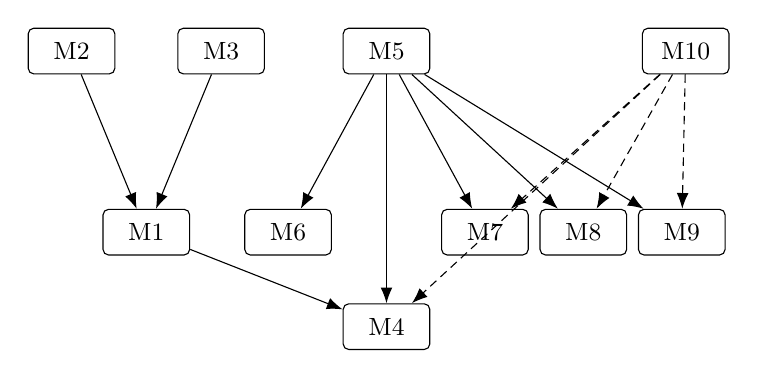
\begin{tikzpicture}[
  unit/.style={draw,rounded corners=2pt,minimum width=1.1cm,minimum height=0.58cm},
  >={Latex[length=2mm]}, every node/.style={font=\small}]
\node[unit] (m2) at (-4,3.5) {M2};
\node[unit] (m3) at (-2.1,3.5) {M3};
\node[unit] (m5) at (0,3.5) {M5};
\node[unit] (m10) at (3.8,3.5) {M10};
\node[unit] (m1) at (-3.05,1.2) {M1};
\node[unit] (m6) at (-1.25,1.2) {M6};
\node[unit] (m4) at (0,0) {M4};
\node[unit] (m7) at (1.25,1.2) {M7};
\node[unit] (m8) at (2.5,1.2) {M8};
\node[unit] (m9) at (3.75,1.2) {M9};
\draw[->] (m2) -- (m1);
\draw[->] (m3) -- (m1);
\draw[->] (m1) -- (m4);
\foreach \i in {4,6,7,8,9} {\draw[->] (m5) -- (m\i);}
\foreach \i in {4,7,8,9} {\draw[->,densely dashed] (m10) -- (m\i);}
\end{tikzpicture}
\caption{Boxes are modules. Solid arrows are live-path dependencies. Dashed arrows are dependencies of the offline harness.}
\label{FigUH}
\end{figure}

M10 is an offline application entry point rather than a live behaviour module dependency. Its independent position preserves the S4 boundary; the FR12 and FR14 rows establish why this software-decision module is required.

The decision policy gets the same class of signals in live and offline use. This allows a frozen calibration and detector version to be checked before deployment. It also keeps a test-only label, error log or dataset out of the live result flow.

\section{User Interfaces}

An extension-owned side panel (using the \href{https://developer.chrome.com/docs/extensions/reference/api/sidePanel}{Chrome Side Panel API}) contains all authoritative consent and result controls. An in-page overlay, if added, is only a non-authoritative mirror and cannot collect consent. M2 presents the selected modality and any provider consent disclosure before dispatch. M3 shows the active request's five-state lifecycle, source-tagged evidence, uncertainty, limitations and next verification step. Authoritative consent and result controls reside in an extension-controlled view; webpage text is inert. Keyboard operation, text status labels and contrast are verified by NFT-2 and FT-16 in the V\&V Plan.

\section{Design of Communication Protocols}

\textbf{Image acquisition.} M1 reads only the selected image. If its bytes cannot be read under the current page's permission, M2 offers a separate user action to allow access to that image's HTTPS origin. M1 requests only that origin as an optional host permission, then fetches the selected URL from the extension context with credentials omitted, redirects rejected, cache bypassed and a streaming byte bound. It does not forward arbitrary URLs to the analysis service. Refusal, a redirected URL, expired gesture or unreadable protected resource returns an input-unavailable reason before analysis. M1 tracks concurrent capture leases and removes a permission acquired for these captures when the last lease ends; it does not revoke a pre-existing user grant. The manifest declares HTTPS origins as optional permissions so an exact origin can be requested at runtime; no broad host permission is granted at installation. This separates image acquisition permission from consent to send content to an analysis provider. Chrome documents the distinct scopes of \href{https://developer.chrome.com/docs/extensions/develop/concepts/activeTab}{active-tab access}, \href{https://developer.chrome.com/docs/extensions/develop/concepts/network-requests}{extension network access} and \href{https://developer.chrome.com/docs/extensions/reference/api/permissions}{optional permissions}; FT-1 Case D checks the proposed acquisition path.

\textbf{Applicability.} M7's versioned applicability gate returns supported, unsupported or uncertain, using the selected text and explicitly supplied context. A declared opinion/satire selection is unsupported. Automatic genre recognition requires a released classifier and held-out genre data in the frozen model profile; without those artifacts its result is uncertain. M9 abstains on unsupported or uncertain applicability. There is no claim that benchmark fixture tags recognize genre in real input. Raymond Tao's model gate and held-out opinion/satire results are a prerequisite to enabling directional text output; a missed FR4 gate requires the SRS scope decision with the TA, as the V\&V Plan states.


M1 transports request-scoped commands to the team service using the SRS S.5 analysis envelope over an authenticated encrypted connection. M5 validates the session and request key independently of caller-supplied identifiers. The MIS shared types are internal abstractions; the transport adapter preserves all SRS fields. Worker events are internal and cannot be submitted as trusted events by a webpage or client.

\section{Database Design}

Live checks use no persistent raw-content database. M6 tracks transient references and worker leases in memory; M5 retains only safe delivery records. Offline M10 records licensed benchmark identities, configurations and outcomes in run artifacts, without accessing live selections. The SRS cleanup bound concerns logical release of application-owned references, not forensic erasure.

\section{Timeline}

Table~\ref{TblSchedule} is the proposed implementation plan from this review to the Revision 0 demonstration. Dates are targets, not completion claims. Owners follow the existing team responsibilities; each reviewer is a different member. The January 18 design freeze precedes the February 1--12 demonstration window. The Nov 23--Dec 4 proof-of-concept window follows the current V\&V Plan.

\begin{longtable}{@{}p{0.15\linewidth}p{0.21\linewidth}p{0.56\linewidth}@{}}
\caption{Module implementation and integration schedule}\label{TblSchedule}\\
\toprule Target window & Owner; reviewer & Deliverable, dependency and confidence check \\ \midrule
\endfirsthead
\toprule Target window & Owner; reviewer & Deliverable, dependency and confidence check \\ \midrule
\endhead
Nov 19--27 & M1: Calvin Salsali; Jaden Moore & Host bridge, scoped capture and trusted side panel; M4's input-limit interface is the prerequisite, with transport stubs developed in parallel. Exercise restricted pages, cross-origin images and encrypted service transport (FT-1). \\
Nov 19--27 & M4: Jaden Moore; Richard Han & Stateless validator; no module prerequisite. Check all nine input classes, Unicode code points, media headers and decoding bounds (FT-2--FT-4). \\
Nov 19--Dec 4 & M6: Richard Han; Jaden Moore & Memory ownership, lease revocation and cleanup receipts; no module prerequisite. Verify no raw disk/log writes and release after each terminal outcome (NFT-4, UT-C5). \\
Nov 23--Dec 11 & M7: Raymond Tao; Richard Han & Text detector and applicability profile; freeze licensed model artifacts. Unit-check signal locators and unavailable/unsupported applicability; record held-out genre evidence before directional release (FT-8--FT-9). \\
Nov 23--Dec 11 & M8: Raymond Tao; Richard Han & Visual detector and provenance parsers; freeze licensed model artifacts. Check original, metadata-absent and inconsistent images, plus parser failure (FT-6). \\
Nov 30--Dec 11 & M9: Raymond Tao; Jaden Moore & Frozen calibration and abstention profile; use versioned M7/M8 signal fixtures. Verify margin boundaries, missing signals and no-guarantee wording (FT-7--FT-9). \\
Nov 30--Dec 18 & M10: Richard Han; Raymond Tao & Replay harness using M4 and M7--M9. Recompute metrics from all eligible outcomes, audit split leakage and subgroup counts, and independently replay the frozen run (FT-15, NFT-1, NFT-7, NFT-10). \\
Dec 7--18 & M2: Calvin Salsali; Richard Han & Selection/consent workflow on M1. Verify approval binds one item and route, decline sends nothing and stale consent is rejected (FT-1, FT-11). \\
Dec 7--18 & M3: Calvin Salsali; Jaden Moore & Result card on M1. Check all status variants, keyboard controls, false-positive warning and late-result suppression (FT-5, FT-10, FT-14, FT-16). \\
Dec 7--Jan 8 & M5: Jaden Moore; Richard Han & Coordinator on M4 and M6--M9; integrate stubs before real models. Exhaust lifecycle guards, timeout/cancel races and ten-request isolation (FT-10, FT-13--FT-14, UT-C4). \\
Jan 4--15 & Jaden Moore; Calvin Salsali & Integrate M1--M10 and run the stub system suites, privacy checks, accessibility and static analysis in PR CI. Richard Han checks cleanup independently; Raymond Tao runs the real-model performance and fairness gates. \\
Jan 18 & Jaden Moore; Richard Han & Freeze Design Revision 0: match MG/MIS to implemented interfaces, trace every requirement and record passed, failed and blocked tests. Resolve changed scope with the TA before claiming acceptance. \\
Jan 19--29 & Calvin Salsali, Raymond Tao, Jaden Moore, Richard Han & Prepare Rev 0 build on the declared reference host. Jaden checks latency, availability and concurrency; Richard replays benchmark/privacy evidence; Calvin checks installation and keyboard flow; Raymond signs the model release profile. Each defect returns to its module owner. \\
Feb 1--12 & Calvin Salsali, Raymond Tao, Jaden Moore, Richard Han & Demonstrate the integrated Rev 0 build and record feedback. Release requires applicable V\&V gates; blocked detector gates stay visibly inconclusive or require an approved scope revision. \\
\bottomrule
\end{longtable}

Jaden Moore owns CI wiring. This follow-up adds a specification-check workflow for the existing eight SRS/HA checks and the MG/MIS consistency audit; the LaTeX workflow already compiles documentation. Product unit tests, static analysis and coverage gates in the V\&V Plan must be added as the modules land. The repository administrator must require successful checks in branch protection; a workflow file alone does not enforce a merge block. The final usability study and complete V\&V report remain later milestones.

\section{Generative AI Use Disclosure}

This section records the AI tools used to prepare and review the design and the checks performed on AI-generated content.

\subsection{AI Tools Used}

\noindent OpenAI Codex (GPT-6), Claude Fable 5.2 and Claude Opus 5.5 were used for drafting and revising this document and for ensuring consistency with the course checklists and the contracts in the team's previous documents.

\subsection{How and Where Used}

\noindent Calvin Salsali used OpenAI Codex (GPT-6, November 2026) to draft the module descriptions, uses diagram, trace tables and companion interface contracts from the team's development plan, SRS, Hazard Analysis, V\&V Plan and course checklists.

\medskip\noindent Richard Han used Claude Fable 5.2 and Claude Opus 5.5 to revise the document, check it against the course checklists, and check its consistency with the team's previous documents.

\medskip\noindent Jaden Moore used OpenAI Codex (GPT-6, November 2026) to review the MG and MIS against the milestone rubric and revise the implementation schedule, traceability and interface contracts.

\subsection{Verification of AI-Generated Content}

\noindent The team read through the full document and checked the AI-generated content for correctness and consistency. Module names, secrets, requirement identifiers, hazard identifiers and symbolic constants were compared against the SRS, Hazard Analysis, V\&V Plan and course checklists, and any errors or inconsistencies were corrected by hand.

\medskip\noindent As an extra check, the AI tools were also asked to review their own generated content against the same sources. Any issues raised in that review were checked by the team before changes were accepted.

\medskip\noindent The follow-up review ran the SRS and Hazard Analysis specification tests, checked MG/MIS traceability and interface consistency, and rebuilt and inspected both PDFs.

\newpage{}

\bibliographystyle {plainnat}
\bibliography{../../../refs/References}

\end{document}
